%\documentclass[
  bibliography=totoc,     % Literatur im Inhaltsverzeichnis
  captions=tableheading,  % Tabellenüberschriften
  titlepage=firstiscover, % Titelseite ist Deckblatt
]{scrartcl}

% Paket float verbessern
\usepackage{scrhack}

% Warnung, falls nochmal kompiliert werden muss
\usepackage[aux]{rerunfilecheck}

% unverzichtbare Mathe-Befehle
\usepackage{amsmath}
% viele Mathe-Symbole
\usepackage{amssymb}
% Erweiterungen für amsmath
\usepackage{mathtools}

% Fonteinstellungen
\usepackage{fontspec}
% Latin Modern Fonts werden automatisch geladen
% Alternativ zum Beispiel:
%\setromanfont{Libertinus Serif}
%\setsansfont{Libertinus Sans}
%\setmonofont{Libertinus Mono}

% Wenn man andere Schriftarten gesetzt hat,
% sollte man das Seiten-Layout neu berechnen lassen
\recalctypearea{}

% deutsche Spracheinstellungen
\usepackage[ngerman]{babel}


\usepackage[
  math-style=ISO,    % ┐
  bold-style=ISO,    % │
  sans-style=italic, % │ ISO-Standard folgen
  nabla=upright,     % │
  partial=upright,   % │
  mathrm=sym,        % ┘
  warnings-off={           % ┐
    mathtools-colon,       % │ unnötige Warnungen ausschalten
    mathtools-overbracket, % │
  },                       % ┘
]{unicode-math}

% traditionelle Fonts für Mathematik
\setmathfont{Latin Modern Math}
% Alternativ zum Beispiel:
%\setmathfont{Libertinus Math}

\setmathfont{XITS Math}[range={scr, bfscr}]
\setmathfont{XITS Math}[range={cal, bfcal}, StylisticSet=1]

% Zahlen und Einheiten
\usepackage[
  locale=DE,                   % deutsche Einstellungen
  separate-uncertainty=true,   % immer Unsicherheit mit \pm
  per-mode=symbol-or-fraction, % / in inline math, fraction in display math
]{siunitx}

% chemische Formeln
\usepackage[
  version=4,
  math-greek=default, % ┐ mit unicode-math zusammenarbeiten
  text-greek=default, % ┘
]{mhchem}

% richtige Anführungszeichen
\usepackage[autostyle]{csquotes}

% schöne Brüche im Text
\usepackage{xfrac}

% Standardplatzierung für Floats einstellen
\usepackage{float}
\floatplacement{figure}{htbp}
\floatplacement{table}{htbp}

% Floats innerhalb einer Section halten
\usepackage[
  section, % Floats innerhalb der Section halten
  below,   % unterhalb der Section aber auf der selben Seite ist ok
]{placeins}

% Seite drehen für breite Tabellen: landscape Umgebung
\usepackage{pdflscape}

% Captions schöner machen.
\usepackage[
  labelfont=bf,        % Tabelle x: Abbildung y: ist jetzt fett
  font=small,          % Schrift etwas kleiner als Dokument
  width=0.9\textwidth, % maximale Breite einer Caption schmaler
]{caption}
% subfigure, subtable, subref
\usepackage{subcaption}

% Grafiken können eingebunden werden
\usepackage{graphicx}

% schöne Tabellen
\usepackage{tabularray}
\UseTblrLibrary{booktabs, siunitx}

% Verbesserungen am Schriftbild
\usepackage{microtype}

% Literaturverzeichnis
\usepackage[
  backend=biber,
]{biblatex}
% Quellendatenbank
\addbibresource{lit.bib}
\addbibresource{programme.bib}

% Hyperlinks im Dokument
\usepackage[
  german,
  unicode,        % Unicode in PDF-Attributen erlauben
  pdfusetitle,    % Titel, Autoren und Datum als PDF-Attribute
  pdfcreator={},  % ┐ PDF-Attribute säubern
  pdfproducer={}, % ┘
]{hyperref}
% erweiterte Bookmarks im PDF
\usepackage{bookmark}

% Trennung von Wörtern mit Strichen
\usepackage[shortcuts]{extdash}

\author{%
  Vincent Wirsdörfer\\%
  \href{mailto:vincent.wirsdoerfer@udo.edu}{authorA@udo.edu}%
  \and%
  Joris Daus\\%
  \href{mailto:joris.daus@udo.edu}{authorB@udo.edu}%
}
\publishers{TU Dortmund – Fakultät Physik}


%\begin{document}

\section{Fehlerrechnung}
\label{sec:Fehlerrechnung}

Alle im Protokoll vermerkten Mittelwerte lassen sich über die folgende Formel berechnen:

\begin{equation}
\label{eqn:Mittelwert}
    \bar{x} = \frac{1}{N}\sum_{i=1}^N x_i
\end{equation}

\noindent Zudem lässt sich der dazugehörige Fehler des Mittelwerts wie folgt berechnen:

\begin{equation}
\label{eqn:Mittelwertfehler}
    \increment \bar{x} = \sqrt{\frac{1}{N\left(N-1\right)}\sum_{i=1}^N \left(x_i - \bar{x}\right)²}
\end{equation}

\noindent Entsteht ein neuer Fehler durch bereits fehlerbehaftete Größen, so wird die Gauß'sche Fehlerfortpflanzung angewendet:

\begin{equation}
\label{eqn:Fehlerfortpflanzung}
    \increment f = \sqrt{\sum_{i=1}^N \left(\frac{\partial f}{\partial x_i}\right)²\cdot\left(\increment x_i\right)²}
\end{equation}


\section{Auswertung}
\label{sec:Auswertung}

Zu Beginn der Auswertung, soll die Zeitkonstante $\tau$ eines RC-Gliedes durch die Analyse eines Auf- beziehungsweise Entladevorgangs
des Kondensators bestimmt werden. Dazu werden bei Beobachtung des Entladevorgangs zugehörige Wertepaare der Zeit $t$ und der Kondensatorspannug $U_C(t)$
entnommen und grafisch dargestellt:\footnote{Die dazugehörigen Werte befinden sich in Tabelle \ref{tab:t-U}}

\begin{figure}[H]
    \centering
    \includegraphics[height=7.5cm]{Entladungskurve.pdf}
    \caption{Entladungsvorgang des Plattenkondensators}
    \label{fig:Entladungskurve}
\end{figure}

\noindent Mit Hilfe von Gleichung \eqref{eqn:Entladung} und der Abbildung \ref{fig:Entladungskurve} lässt sich die lineare Ausgleichsrechnung 

\begin{equation}
    \ln\left(\frac{U_C}{U_0}\right) = \underbrace{-\frac{1}{RC}}_m \cdot t + b
\end{equation}

\noindent nachvollziehen. Der Wert für die Zeitkonstante $\tau$ ergibt sich somit aus dem negativen Kehrwert der Steigung $m$.\\
Der gemessene Parameter der Ausgleichsgerade lauten demnach:

\begin{equation}
    RC = \left(1.52 \pm 0.06\right)\,\cdot 10^{-3}\,\unit{\second}
\end{equation}

\noindent Die nächste Methode zur Bestimmung der Zeitkonstante unterliegt dem Zusammenhang zwischen der Frequenz $f$ und dem 
Amplitudenverhältnis $\sfrac{U_C}{U_0}$. Dementsprechend wird die Menge der Wertpaare ${\sfrac{U_C}{U_0},f}$ sowie eine 
nicht-lineare Ausgleichsgerade grafisch aufgetragen:\footnote{Die Werte für dieses Diagramm entstammen Tabelle \ref{tab:f-A-a}.}

\begin{figure}
    \centering
    \includegraphics[height=7.5cm]{Amplitudenspannung.pdf}
    \caption{Zeitlicher Verlauf des Amplitudenverhältnis.}
    \label{fig:Amplitudenverlauf}
\end{figure}

\noindent Durch korrektes der Umstellen der Gleichung \eqref{eqn:Phase_Amplitude} kann die Zeitkonstante bestimmt werden:

\begin{equation}
    RC = \left(2.19 \pm 0.18\right)\,\cdot 10^{-3}\,\unit{\second}
\end{equation}
\newpage
\noindent Neben der Amplitude $U_C$ der Kondensatorspannug ist auch die Phasenverschiebung $\varphi$ zwischen Generator- und
Kondensatorspannug abhängig von der Ausgangsfrequenz $f$. Dieser Zusammenhang wird in der nächsten Methode ausgenutzt, wobei 
die Menge der Wertepaare ${\varphi , f}$ grafisch aufgetragen werden: 

\begin{figure}[H]
    \centering
    \includegraphics[height=7.5cm]{phi(f).pdf}
    \caption{Zusammenhang zwischen der Frequenz $f$ und der Phasenverschiebung $\varphi$.}
    \label{fig:Phasenverschiebung}
\end{figure}

\noindent Der konkrete mathematische Zusammenhang lässt sich an 
Gleichung \eqref{eqn:Phase_Amplitude} ablesen. Durch äquivalentes Umformen ebenfalls dieser Gleichung kann somit die Zeitkonstante
berechnet werden. Eine Teilmenge\footnote{Warum hier nur eine Teilmenge der Werte verwendet wurde, wird in der Diskussion behandelt} der dafür verwendeten Werte befindet sich in Tabelle \ref{tab:f-A-a}
Daraus resultiert die folgende Zeitkonstante:

\begin{equation}
    RC = \left(... \pm ...\right)\,\cdot 10^{-x}\,\unit{\second}
\end{equation}


\noindent Die Menge der Wertepaare ${\sfrac{A(\omega)}{U_0},\varphi}$ aus Tabelle \ref{tab:f-A-a} können jedoch nicht nur in ein kartesisches Koordinatensystem eingetragen, sondern
auch als Polarplot dargestellt werden. Dies sähe dann folgendermaßen aus:

\begin{figure}[H]
    \centering
    \includegraphics[height=7.5cm]{polar2.pdf}
    \caption{Polarplot der Phasenverschiebung $\varphi$ und Relativamplitude $\sfrac{A(\omega)}{U_0}$.}
    \label{fig:polar}
\end{figure}

\noindent Zuletzt wird gezeigt, dass der RC-Kreis auch als Integrator verwendet. Wie in der Theorie postuliert muss dafür die Kreisfrequenz $\omega$
wesentlich größer als der Kehrwert der Zeitkonstante $\sfrac{1}{RC}$ sein. Dies kann mittels des abfotografierten Oszilloskops geprüft werden:

\begin{figure}[H]
    \begin{subfigure}{0.5\textwidth}
        \centering
        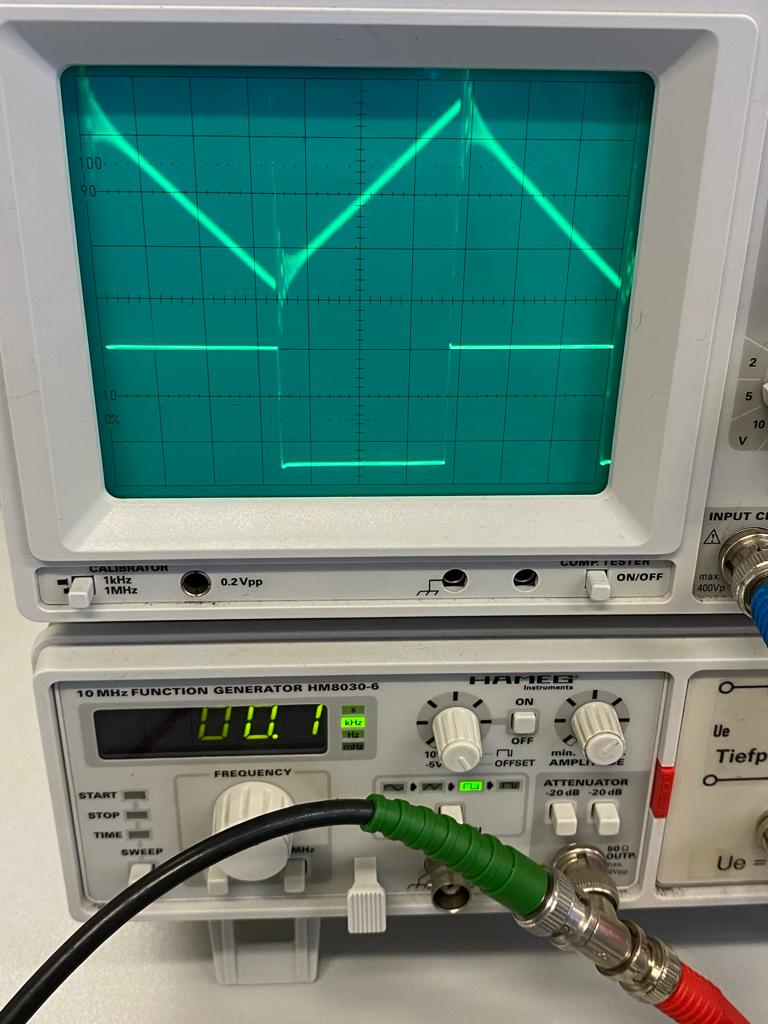
\includegraphics[width=6.5cm]{./content/Rechtecksspannung.jpg}
        \caption{Rechtecksspannung}
        \label{fig:Rechteck}
    \end{subfigure}
    \begin{subfigure}{0.5\textwidth}
        \centering
        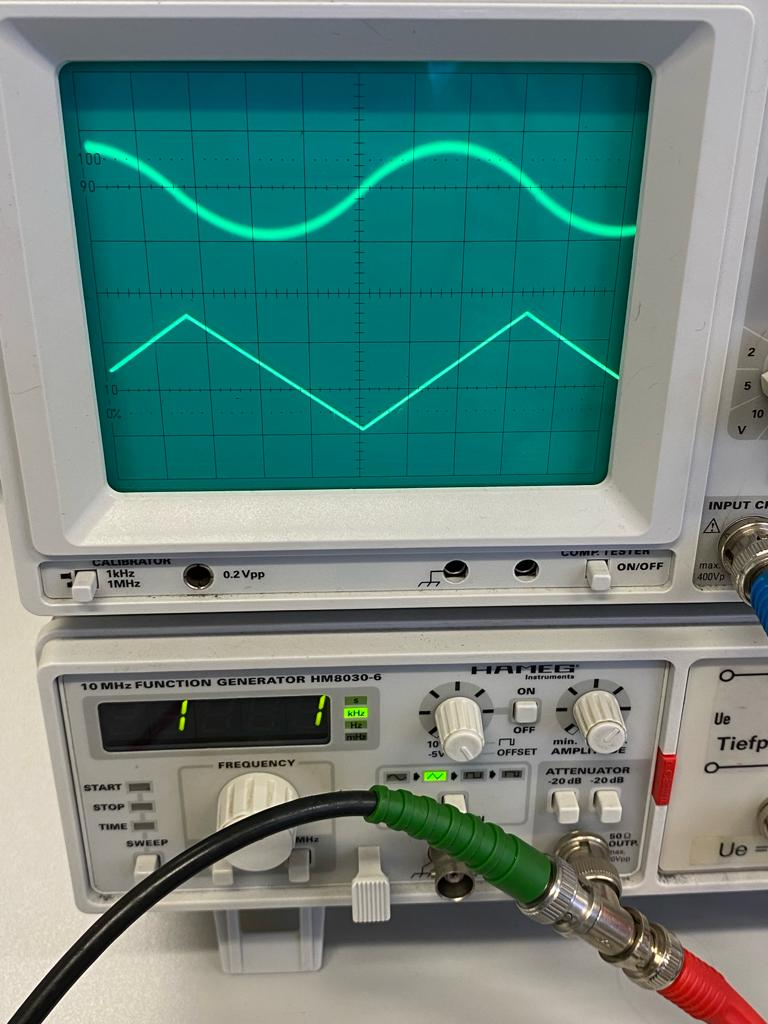
\includegraphics[width=6.5cm]{./content/Dreiecksspannung.jpg}
        \caption{Dreiecksspannung}
        \label{fig:Rechteck}
    \end{subfigure}
    \begin{subfigure}{0.5\textwidth}
        \centering
        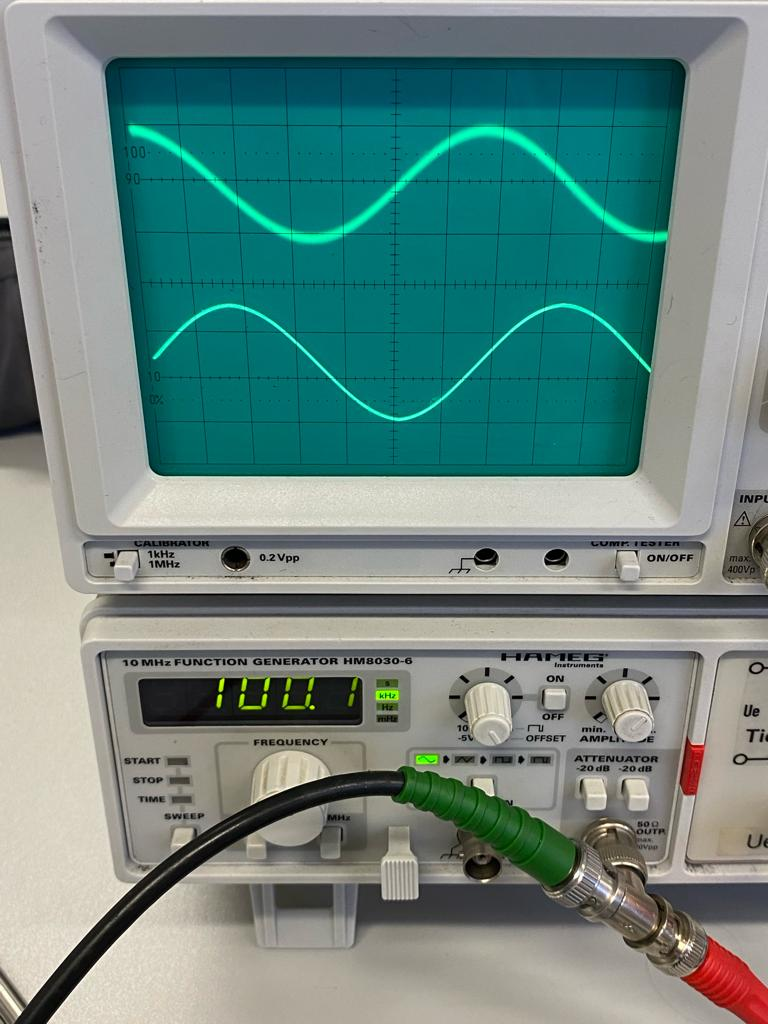
\includegraphics[width=6.5cm]{./content/Sinusspannung.jpg}
        \caption{Sinusspannung}
        \label{fig:Rechteck}
    \end{subfigure}
\end{figure}
\noindent
Das Oszilloskop auf den Fotos bestätigt, dass der RC-Kreis unter der Voraussetzung $\omega >> \frac{1}{RC}$ als Intergrator dienen kann. 
%\end{document}
